\documentclass[a4paper,11pt]{extarticle}
% \usepackage[english,vietnam]{babel}
\usepackage[utf8]{vntex}
\usepackage{booktabs}
% \usepackage[T1]{fontenc}
%\usepackage[utf8]{inputenc}
%\usepackage[francais]{babel}
\usepackage{a4wide,amssymb,epsfig,latexsym,multicol,array,hhline,fancyhdr}
\usepackage{tabularx} % in the preamble
\usepackage{mathtools}
\usepackage{listings}
\usepackage{minted}
%%%%%%%%%%%%
\usepackage{verbatimbox}
\usepackage{lscape}
\usepackage{pdflscape}
%%%%%%%%%%%%
\usepackage{fancyvrb}
\usepackage{minted}
\usepackage{amsmath}
\usepackage{nicefrac}
\usepackage{tabularx}
\usepackage{lastpage}
\usepackage[lined,boxed,commentsnumbered]{algorithm2e}
\usepackage{color}
\usepackage{graphicx}							% Standard graphics package
\usepackage{array}
\usepackage{tabularx, caption}
\usepackage{multirow}
\usepackage{multicol}
\usepackage{rotating}
\usepackage{graphics}
\usepackage[left=3.00cm, right=2.00cm, top=2.50cm, bottom=4.00cm]{geometry}
\usepackage{setspace}
\usepackage{epsfig}
\usepackage{tikz}
\usetikzlibrary{arrows,backgrounds}
\usepackage[unicode]{hyperref}
\hypersetup{urlcolor=blue,linkcolor=black,citecolor=black,colorlinks=true} 
%\usepackage{pstcol} 								% PSTricks with the standard color package
% Table package
\usepackage{array}
\newcolumntype{L}[1]{>{\raggedright\let\newline\\\arraybackslash\hspace{0pt}}m{#1}}
\newcolumntype{C}[1]{>{\centering\let\newline\\\arraybackslash\hspace{0pt}}m{#1}}
\newcolumntype{R}[1]{>{\raggedleft\let\newline\\\arraybackslash\hspace{0pt}}m{#1}}

% Use case table
%%%%%%%%%%%%%%%%%%%%%%%%%%%%%%%%%%%%%
\newcommand\tabularhead[2]{
\begin{table}[ht]
  \small
%   \caption{<<#1>> use case description}
  \begin{tabular}{|p{0.2\linewidth}|p{0.75\linewidth}|}
    \hline 
    \textbf{Name} & #1 \\
    \hline
    \textbf{Actor} & #2 \\
    \hline}

  \newcommand\addrow[2]{\textbf{#1} &#2\\ \hline}

  \newcommand\addmulrow[2]{ \begin{minipage}[t][][t]{\linewidth}\textbf{#1}\end{minipage}% 
     &\begin{minipage}[t][][t]{\linewidth}
      \begin{enumerate}[wide=0pt] #2   \end{enumerate}
      \smallskip
      \end{minipage} \\ 
      \hline }

  \newenvironment{usecase}{\tabularhead}
{\hline\end{tabular}\end{table}}
%%%%%%%%%%%%%%%%%%%%%%%%%%%%%%%%%%%%%
%%%%%%%%%%%%%%%%%%%%%%%%%%%%%%%%%%%%%
\everymath{\color{blue}}
\everydisplay{\color{blue}}
\def\m@th{\normalcolor\mathsurround\z@}
\usepackage{enumitem}
\setlist[itemize]{noitemsep, topsep=0pt}
\setlist[enumerate]{nosep}

%%%%%%%%%%%%%%%%%%%%%%%%%%%%%%%%%%%%%
%\usepackage{fancyhdr}

\setlength{\headheight}{40pt}
\setlength{\parindent}{0pt}
\setlength{\parskip}{5pt}
\linespread{1.2}
\pagestyle{fancy}
\fancyhead{} % clear all header fields
\fancyhead[L]{
 \begin{tabular}{rl}
    \begin{picture}(25,15)(0,0)
    \put(0,-8){
\includegraphics[width=10mm, height=10mm]{hcmut.png}}
    %\put(0,-8){\epsfig{width=10mm,figure=hcmut.eps}}
   \end{picture}&
	%
\includegraphics[width=8mm, height=8mm]{hcmut.png} & %
	\begin{tabular}{l}
		\textbf{\bf \ttfamily Ho Chi Minh City University of Technology}\\
		\textbf{\bf \ttfamily Faculty of Computer Science \& Engineering}
	\end{tabular} 	
 \end{tabular}
}
\fancyhead[R]{
	\begin{tabular}{l}
		\tiny \bf \\
		\tiny \bf 
	\end{tabular}  }
\fancyfoot{} % clear all footer fields
\fancyfoot[L]{\scriptsize \ttfamily Computer Network -  2020-2021}
\fancyfoot[R]{\scriptsize \ttfamily Page {\thepage}/\pageref{LastPage}}
\renewcommand{\headrulewidth}{0.3pt}
\renewcommand{\footrulewidth}{0.3pt}
\usepackage{datetime}
\newdateformat{monthyeardate}{%
  \monthname[\THEMONTH] \THEYEAR}

%%%
\setcounter{secnumdepth}{4}
\setcounter{tocdepth}{3}
\makeatletter
\newcounter {subsubsubsection}[subsubsection]
\renewcommand\thesubsubsubsection{\thesubsubsection .\@alph\c@subsubsubsection}
\newcommand\subsubsubsection{\@startsection{subsubsubsection}{4}{\z@}%
                                     {-3.25ex\@plus -1ex \@minus -.2ex}%
                                     {1.5ex \@plus .2ex}%
                                     {\normalfont\normalsize\bfseries}}
\newcommand*\l@subsubsubsection{\@dottedtocline{3}{10.0em}{4.1em}}
\newcommand*{\subsubsubsectionmark}[1]{}
\makeatother

%\usepackage[variablett]{lmodern}
% \renewcommand{\rmdefault}{\ttdefault}
% \usepackage[LGRgreek]{mathastext}
% \MTgreekfont{lmtt} % no lgr lmvtt, so use lgr lmtt
% \Mathastext
% \let\varepsilon\epsilon % only \varsigma in LGR
% \usepackage{everysel}
% \renewcommand*\familydefault{cmtt}
% \EverySelectfont{%
% \fontdimen2\font=0.4em% interword space
% \fontdimen3\font=0.2em% interword stretch
% \fontdimen4\font=0.1em% interword shrink
% \fontdimen7\font=0.1em% extra space
% \hyphenchar\font=`\-% to allow hyphenation
% }

\begin{document}

\begin{titlepage}
\begin{center}
ĐẠI HỌC QUỐC GIA THÀNH PHỐ HỒ CHÍ MINH \\
TRƯỜNG ĐẠI HỌC BÁCH KHOA \\
KHOA KHOA HỌC VÀ KỸ THUẬT MÁY TÍNH
\end{center}

\vspace{1cm}

\begin{figure}[h!]
\begin{center}

\includegraphics[width=4cm]{hcmut.png}
\end{center}
\end{figure}

\vspace{1cm}


\begin{center}
\begin{tabular}{c}
\multicolumn{1}{l}{\textbf{{\Large MẠNG MÁY TÍNH}}}\\
~~\\
\hline
\\
\multicolumn{1}{l}{\textbf{{\Large Bài tập lớn 1}}}\\
\\
\textbf{{\Huge Quản lý hệ thống }}\\
\textbf{{\Huge thông qua mô hình client-server}}\\
\\
\hline
\end{tabular}
\end{center}

\vspace{1cm}

\begin{table}[h]
\begin{tabular}{rrll}
\hspace{3 cm} & GVHD: & Nguyễn Hồng Nam\\
 & Sinh viên: & Nguyễn Trần Quang Minh & - 1811083 \\
 &          & Thái Văn Nhật	& - 1813381 \\
 &          & Trần Cao Mạnh	& -  \\
 &          & Văn Chấn Dương & - 1811824\\ 
\\
\vspace{2cm}
\end{tabular}
\end{table}

\begin{center}
{\footnotesize Thành phố Hồ Chí Minh,  \monthyeardate\today}
\end{center}
\end{titlepage}


%\thispagestyle{empty}

\newpage
\tableofcontents
\newpage

%%%%%%%%%%%%%%%%%%%%%%%%%%%%%%%%%
%%%%%%%%%%%%%%%%%%%%%%%%%%%%%%%%%
\section{Nội dung, nhiệm vụ và yêu cầu}
\subsection{Nội dung}
Thiết kế các giao thức phục vụ cho việc kiểm tra tài nguyên của các thiết bị trong cùng một hệ thống và hiện thực các giao thức đã thiết kế. \\
Mô hình ứng dụng được thiết kế theo kiến trúc tổng thể như sau:
\begin{figure}[htbp]
    \centering
    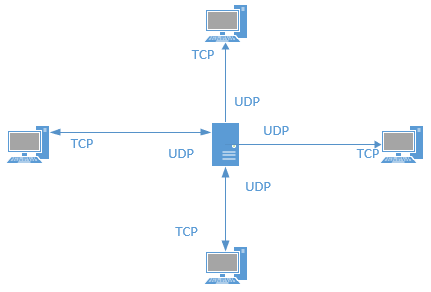
\includegraphics{Model.png}
    \caption{Mô hình giao tiếp giữa client và server}
    \label{fig:my_label}
\end{figure} \\
Nhìn chung, hệ thống có thể được chia thành các phần chính như sau:
\begin{itemize}[noitemsep]
    \item Client: Ứng dụng sẽ lấy các thông số về hệ thống của mình như: Nhiệt độ CPU, dung lượng Disk đang sử dụng, dung lượng RAM đang sử dụng, và các thông số khác. Sau đó client sẽ gửi các thông số này về server để tính toán và ra quyết định. Những dữ liệu này được gửi định kỳ về cho server thông qua kết nối TCP. Thời gian định kỳ này được server gửi cho client.
    \item Server: Trung tâm lưu trữ, mọi dữ liệu sẽ được server lưu giữ và tính toán và hiển thị số liệu tổng hợp.
\end{itemize}

\subsection{Nhiệm vụ}
Hiện thực các Client, Server và ứng dụng tổng hợp số liệu với các ràng buộc sau: 
\begin{itemize}[noitemsep]
    \item Client: client đăng ký tham gia vào hệ thống bằng cách gửi một gói tin gồm các thông số: \emph{Tên, IP, UPD port} để nhận thông báo từ server (nếu có), \emph{ngày giờ hiện tại} lên server theo giao thức \emph{TCP}. Sau khi nhận được gói tin đăng ký Server phải gửi lại thông báo đăng ký thành công hay thất bại cho client. Nếu thành công thì trong gói tin gửi về cho client phải có \emph{ID} của client và \emph{thời gian định kỳ} gửi các thông số lên server và \emph{TCP port} để client gửi gói tin lên hệ thống. Nếu không thành công thì trong gói tin có mã lỗi và nội dung lỗi. \\
    Sau khi có các thông tin trên client sẽ gủi dữ liệu lên hệ thống theo định kỳ thời gian đã được thiết lập từ gói tin phản hồi đăng ký của server thông qua giao thức TCP và port của server. \\
    Nếu client nhận được các gói tin UDP được gửi từ server về việc thiết lập lại các thông số gửi dữ liệu gồm: TCP Port và thời gian định kỳ thì client phải hiệu chỉnh cho phù hợp.    
    \item Server: Server nhận các gói tin đăng ký của client và sinh ra một \emph{Unit ID} cho client và gửi về client kèm theo các thông số cần thiết. Sau khi nhận được các dữ liệu của client server sẽ tổng hợp và hiển thị lên cho người dùng xem. Server có thể gửi \emph{UDP message} cho tất cả hoặc một vài client cụ thể để thay đổi các thông số thiết lập.
\end{itemize}

\subsection{Yêu cầu}
\begin{itemize}[noitemsep]
    \item Định nghĩa các bộ giao thức cho ứng dụng.
    \item Hiện thực Client đơn giản đọc dữ liệu của máy tính gồm nhiệt độ CPU, thông số sử dụng ổ cứng, RAM và gửi về cho client theo giao thức đã được định nghĩa.
    \item Server phải đảm bảo được việc sử lý dữ liệu của nhiều client cùng một lúc.
    \item Server phải hiển thị các kết quả tổng hợp cho người dùng xem
\end{itemize}
%%%%%%%%%%%%%%%%%%%%%%%%%%%%%%%%%
\section{Phân tích nội dung, nhiệm vụ và yêu cầu}
Các giao thức được thiết kế sẽ phục vụ cho việc kiểm tra tài nguyên của các thiết bị trong cùng một hệ thống. Do vậy việc xác định địa chỉ IP của các thành phần trong hệ thống là xác định địa chỉ của các host trong nội bộ subnet. Hệ thống bao gồm các thành phần cụ thể sau:
\begin{enumerate}[noitemsep]
    \item Server: Một host trong hệ thống chịu trách nhiệm làm nơi quản lý các thông tin tài nguyên mà các thiết bị trong hệ thống sẽ gửi về.
    \item Các client: Các host trong hệ thống, khi có nhu cầu sẽ sử dụng ứng dụng để kết nối với server để gửi thông tin liên quan đến tài nguyên của mình.
\end{enumerate}
Yêu cầu chỉ ra cần phải thiết kế client có khả năng kết nối với server thông qua bộ giao thức được định nghĩa sẵn, dựa trên nhiệm vụ được đề ra, bộ giao thức có thể được định nghĩa như sau: 
\subsection{Giao thức}
- Format của payload của gói tin: \\
\framebox{\texttt{[16 bytes: msg's length][5 bytes: command abbreviation][data]}} \\
Trong đó:
\begin{itemize}[noitemsep]
    \item \texttt{[msg's length]} là độ dài của payload, chiếm 16 bytes trong payload.
    \item \texttt{[command abbreviation]} là 5 bytes xác định loại message để client và server xử lý.
    \item \texttt{[data]} là phần còn lại của payload, chứa các dữ liệu tuỳ vào loại message.
\end{itemize}

% - Client: 
%     Send its registering information through TCP, including its Name, IP addr, UDP port (to receive server's info), current date/time 
    
%     Khi mở được đường kết nối được với server,  client sẽ gửi một gói tin TCP chứa thông tin đăng ký với server bao gồm các trường dưới dạng format \texttt{json} như sau:
%     \begin{itemize}[noitemsep]
%         \item \texttt{"name"} Xác định tên của client.
%         \item \texttt{"ip_addr"} Xác định IP address của client.
%         \item \texttt{"UDP_port"} Xác định UDP port mà client dùng để nhận các gói tin UDP từ server báo về.
%         \item \texttt{"current_time"} Xác định thời điểm tạo thông tin để gửi đăng ký.
%     \end{itemize}
% Server:
%     - After receiving registering information from the client, server send the unit id of client, the tcp port and the interval to the client.
%     - Server can send message to the client through the udp port client sent.
%     - Reply to registering packets:
%         "!SUCC + [info]"
%         or "!FAIL + [error]"
%     - When sending the change in interval time, if within 5s the server doesn't receive the received change message from the client then the server will resend the change.
% Clean disconnection:
% Sent the message "!DISC" to confirm clients' disconnection.        

% Consider changing this, maybe the length is redundant.
\subsubsection{Quá trình đăng ký:}
Để bắt đầu quá trình gửi thông tin tài nguyên, client cần phải tạo đường TCP connect tới server thông qua địa chỉ IP và port của server được cung cấp từ đầu. \\
Gói tin đăng kí của client có cú pháp như sau: \framebox{\texttt{[msg's length]!RGTR[info]}} \\
Phía server có các gói tin xác nhận như sau:
\begin{itemize}
    \item Gói tin xác nhận đăng ký thành công (khi đúng cú pháp và đầy đủ các trường ở dữ liệu): \framebox{\texttt{[msg's length]!SUCC[info]}}
    \item Gói tin xác nhận đăng ký không thành công (connect tới được nhưng không đăng ký được):
\framebox{\texttt{[msg's length]!FAIL[info]}}
\end{itemize}
Đối với gói tin đăng ký của client, \texttt{[info]} bao gồm các field sau (bắt buộc phải có format \texttt{json} để server parse, không có thì cũng xem như đăng ký không thành công).
\begin{itemize}[noitemsep]
    \item \texttt{"name"} : tên của client (thường là device name)
    \item \texttt{"ip"} : địa chỉ ip của client
    \item \texttt{"UDP\_port"} : port mà client dùng để nhận gói tin thông báo cập nhật từ server.
    \item \texttt{"time"}: thời gian client gửi thông tin đăng ký.
\end{itemize}
Đối với gói tin xác nhận đăng ký thành công của server, \texttt{[info]} bao gồm các field sau (bắt buộc phải có format \texttt{json} để client parse):
\begin{itemize}[noitemsep]
    \item \texttt{"client\_id"} : UUID của client do server cấp.
    \item \texttt{"tcp\_port"} : TCP port của server để client gửi thông tin lên.
    \item \texttt{"interval"} : Khoảng thời gian định kỳ mà client phải gửi lên cho server.
\end{itemize}
Đối với gói tin đăng ký không thành công, \texttt{[info]} bao gồm thông tin lỗi. \\
\textbf{Ngữ cảnh:} \\
Client kết nối tới server lần đầu thông qua địa chỉ \texttt{(ip\_addr, port)} của server, có thể có các trường hợp sau xảy ra:
\begin{enumerate}[noitemsep]
    \item Client tạo đường connect thành công tới server:
    \begin{enumerate}[noitemsep]
        \item Trường hợp client gửi đúng cú pháp cho server để đăng ký: \\
        Server gửi Gói tin đăng ký thành công về cho client. Từ đây server listen trên 1 port đã chỉ định cho client gửi thông tin về. 
        \item Trường hợp client không gửi đúng cú pháp cho server: \\
        Trường hợp này thì server nhận biết bằng cách parse lỗi phần data, sau đó server sẽ gửi một gói tin báo lỗi về cho client với cú pháp như ở phía trên.
    \end{enumerate}
    \item Client không tạo được đường connect tới server:
    \begin{enumerate}[noitemsep]
        \item Server không hoạt động: Sau một khoảng thời gian timeout, client sẽ ngừng chương trình.
        \item Client lỗi: client gặp lỗi gì sẽ báo lỗi đó.
    \end{enumerate}
\end{enumerate}

\subsubsection{Quá trình gửi thông tin:}
Gói tin chứa thông tin tài nguyên có cú pháp như sau: \framebox{\texttt{[msg's length]!INFO[info]}} \\
Gói tin xác nhận việc gửi info thành công của server có cú pháp như sau: \framebox{\texttt{[!INFO: RECEIVED]}}  \\
\texttt{[info]} của client: \\
Hiện tại client có khả năng thu thập các thông tin sau để gửi về cho server: Average CPU's utilization (\% CPU sử dụng trung bình tại một thời điểm), Disk drive's usage (\% dung lượng đĩa đã sử dụng), RAM's usage (\% RAM đã sử dụng tại một thời điểm).  \\
% (CPU temp hiện tại chưa lấy một cách hoàn chỉnh được).
% CPU temp: using psutil (linux), using WMI and OpenHardwareMonitor (windows)
% Disk drive's usage: using psutil
% RAM's usage: using psutil
\textbf{Ngữ cảnh}: \\
Client gửi info cho server thông qua địa chỉ đã được quy định ngay đợt connect đầu tiên, từ đây client cứ hết interval sẽ gửi thông tin về cho server. \\
Nếu server nhận được thì server trả confirmation về cho client. \\ 
Khi có sự cố mà server không gửi được gói tin confirmation về cho client hoặc client gửi cho server không được thì error raised, kết nối giữa client và server sẽ bị ngắt.

\subsubsection{Quá trình ngắt kết nối:}
Để đảm bảo cho client ngắt kết nối một cách an toàn và thuận tiện hơn cho quá trình quản lý của server, giao thức về việc ngắt kết nối một cách an toàn là cần thiết. \\
Gói tin ngắt kết nối của client có cú pháp như sau:
\framebox{\texttt{[msg's length]!DISC}}
Gói tin xác nhận quá trình ngắt kết nối của server có cú pháp như sau: \framebox{\texttt{[!DISC: RECEIVED]}}  \\
\textbf{Ngữ cảnh:} \\
Client gửi disconnect message cho server thông qua địa chỉ đã được quy định ngay đợt connect đầu tiên, server khi nhận được sẽ gửi gói tin confirmation về cho client báo việc disconnect là an toàn. \\
Trường hợp client không nhận được gói tin disconnection confirm từ server thì sau 10s sẽ gửi lại 1 lần, chờ tới khi nào server confirm thì mới được disconnect. \\
Trường hợp server không thể nhận gói tin mà client gửi về (server không hoạt động hay đã bị ngắt), khi đó client có thể ngắt kết nối và tắt chương trình.

\subsubsection{Quá trình cập nhật thông tin:}
Server sẽ gửi gói tin UDP chứa các thông tin cần cập nhật cho client, các thông tin liên quan đến quá trình cập nhật như sau: \\
Gói tin cập nhật thông tin từ server gửi cho client có cú pháp như sau: \\
\framebox{\texttt{[msg's length]!UPDT[interval]}} \\
\textbf{Ngữ cảnh:} \\
Server gửi update message cho client (hiện tại một lúc chỉ thao tác gửi cho 1 client cụ thể) thông qua địa chỉ đã được quy định ngay đợt connect đầu tiên, client khi nhận được sẽ cập nhật khoảng thời gian định kỳ gửi thông tin tài nguyên lên cho server, dựa trên thông tin tài nguyên client gửi về mà ta biết client có đổi thành công hay không. \\
Trường hợp client không nhận được gói tin update message từ server thì ta sẽ điều khiển server gửi lại gói tin cập nhật cho client.

\subsection {Các thiết kề về mô hình giao tiếp và hiện thực ứng dụng}
%%%% %TODO
\section{Đánh giá kết quả đạt được}
%%%%% %TODO
\section{Các chức năng mở rộng của hệ thống ngoài các yêu cầu được qui định}
%%%% %TODO
\section{Hướng dẫn sử dụng ứng dụng}
%%% %TODO
%%%%%%%%%%%%%%%%%%%%%%%%%%%%%%%%%
\end{document}   